\documentclass[a4paper]{article}
\usepackage[warn]{mathtext}
\usepackage[utf8]{inputenc}
\usepackage[T2A]{fontenc}

\usepackage[english,russian]{babel}
\usepackage{multicol}
\usepackage{fancyhdr}
\usepackage{graphicx}
\usepackage{microtype}
\usepackage{wrapfig}
\usepackage{amsmath}
\usepackage{floatflt}
\usepackage{geometry} \geometry{verbose,a4paper,tmargin=2cm,bmargin=2cm,lmargin=1.5cm,rmargin=1.5cm}
\usepackage{float}
\usepackage{amssymb}
\usepackage{caption}
\usepackage{epsfig}
\usepackage{newunicodechar}

\begin{document}

\graphicspath{ {pictures/} }

\begin{titlepage}
	\centering
	\vspace{5cm}
    {\scshape\LARGE Московский физико-технический институт\par}
	\vspace{5cm}
	{\scshape\Large Лабораторная работа по общей физике \par}
	\vspace{1cm}
    {\huge\bfseries  9.1 Закон Кюри-Вейса и обменной взаимодействие в ферромагентиках \par}
	\vspace{1cm}
	\vfill
    \begin{flushright}
        {\large выполнил студент Б04-852 группы ФЭФМ}\par
        \vspace{0.3cm}
        {\LARGE Яромир Водзяновский}
    \end{flushright}
	\vfill
Долгопрудный, 2021
% Bottom of the page
\end{titlepage}

\pagestyle{fancy} 
\fancyhead[L]{Закон Кюри-Вейса    $\sim  \hat(\, ^{\circ}  \omega  ^{\circ} \, \hat) \sim$}
% \fancyhead[L]{Закон Кюри-Вейса    $( *{^\circ}< >^{\circ}*)$}
\fancyhead[R]{Современная физика}
\fancyhead[C]{}
\fancyfoot[C]{ \noindent\rule{\textwidth}{0.4pt} \thepage }

\tableofcontents

\newpage



\section{Цель работы}

\begin{itemize}
    
    \item Исследовать температурную зависимость магнитной восприимчивости ферромагнетика в парамагнитной области.
    \item Определить темперутуру Кюри для металлического гадолиния.
    \item Оценить энергию обменного взаимодействия.
\end{itemize}



\section{Теория}

\subsection{Феноменологичная теория.}

\textbf{Парамагнетики} - в-ва, атомы которых обладают нескомпенсированныз магнитным моментом. При присутсвующем внешнем магнитном поле магнитные моменты атомов и свободных электронов
наравленны <<по полю>> (энергитически выгодно), а в его отсутвии - хаотично. \par 
\begin{equation}
    I = \kappa H
\end{equation}
$I$ - намагниченность (магнитный момент единицы обьема), $H$ - внешнее магнитное поле, $\kappa$ - магнитная восприимчивость. \par 

Пусть магнитный момент атома определяется только спином одного электрона. Проекция спина  $\pm \hbar/2$. Проекция спинового-магнитного момента 
$\mu_z = \mp \mu$, $\mu = \mu_b$ - абсолютное значение проекции магнитного момента равная магнетрону Бора. \par 

Под внешним магнитным полем будет расщепление на две возможные энергии:
\begin{equation}
    E_- = - \mu B, \;\;\;\;\; E_+ = +\mu B
\end{equation}

По Больцману отношение элекутронов с энергиями:

\begin{equation}
    \frac{N_+}{N_-} = e^{-\frac{2 \mu B}{k_bT}} \approxeq 1 - \frac{2\mu B}{k_b T}
\end{equation}

Намагниченность вещества определяется разностью числа электронов, магнитные моменты которых орейнтированы по полю или против поля:

\begin{equation}
    \Delta N \approxeq N \frac{\mu H}{k_b T}
\end{equation}

$N = N_- + N_+$ - кол-во неспаренных электронов в единице обьема. 

Магнитный момент в-ва:

\begin{equation}
    I = \mu \Delta N = N \frac{\mu^2}{k_bT}H
\end{equation}

Восприимчивость равна:

\begin{equation}
    \kappa = \frac{I}{H} = N \frac{\mu_b^2}{k_b T}
\end{equation}

Магнитный момент электрона $\mu$ связан с мезаническим моментом: 

\begin{equation}
    \mu = g \mu_b J
\end{equation}

для свободного электрона $g = 2, \; J = S = 1/2$.

Более общее выражение если более одного электрона, \textbf{Закон Кюри}:

\begin{equation}
    \kappa = \frac{N g^2 \mu_b^2 S(S+1)}{3 k_b T} \propto \frac{1}{T}
\end{equation}


\textbf{Ферромагнетики} - в-ва обладающие намагниченностью в отвутсвие внешнего магнитного поля при температуре ниже точки Кюри.
В ферромагнетике есть эффективное магнитное поле $H_э$ описывающее обменную силу. 

\begin{equation}
    H_э = \lambda I
\end{equation}

При температуре выше $T_c$ ферромагнетик является парамагнетиком - тепловое движение разупорядочивает магнитные моменты.
С учетом $H_э$:

\begin{equation}
    I = N \frac{\mu^2 H}{k_b(T - \Theta)}, \;\;\; \Theta = N\frac{g^2 \mu_b^2 S(S+1)}{3 k_b} \lambda
\end{equation}

\textbf{Формула Кюри-Вейса}:

\begin{equation}
    \kappa = N \frac{g^2 \mu_b^2 S(S+1)}{3 k_b (T - \Theta)} \propto \frac{1}{T - \Theta}
\end{equation}

Закон Кюри-Вейсса предпологает наличие дополнительного поля $H_{эфф}$, в отличие от квантово-механического подхода, эта теория приблизительна, но 
правильно указывает на наличие особой точки $\Theta$ фазового перехода. Эта формула неплохо описывает температурную зависимость магнитной восприимчивости парамагнитной фазы.
\par 
При стремлении температуры к $\Theta$ восприимчивость $\kappa$ неограниченно возрастает из-за того, что тепловое движение все меньше препядствует магнитным моментам орейнтироваться в одном направлении.
У парамагнетиков это происходит только при $T \rightarrow 0$. Точка Кюри $T_c$ определяется как темперартура фазового перехода из парамагнитного состояния в ферромагнитное, при темперутуре ниже темпаратуры Кюри 
устанавливается дальний магнитный порядок. В уравнении Кюри-Вейсса $\Theta $ является эти параметром и $\Theta > T_c$.


\subsection{Связь эффективного поля Вейсса с обменным инегралом}

В теории Гейнзенберга-Френкеля энергия обменног взаимодействия атомов $i$ и $j$ выражается:

\begin{equation}
    U_{обм} = -2JS_iS_j
\end{equation}

$U$ - разность между соседними значениями кулоновской энергии для параллельных и антипараллельных спинов $S_i$ и $S_j$, $J$ - коэффициент пропорциональности, т.е. обменный интеграл, величина которого зависит от степени перекрытия распределенных зарядов атомов 
$i$ и $j$ (от степени перекрытия волновых функций электронов). \par 

Какова связь между обменным интегралом $J$ и константой Кюри-Вейсса $\lambda$?  Пусть атом имеет $n$ соседей, и обменное взаимодействие между каждым из них одинаково, а для особо далеких соседей будем считать 
обменный интеграл $J=0$. Энергия переворота спигна в присутсвии других спинов будет вдвое больше обменной жнергии системы  с неопределенной ориентацией спина, тк $U_{\upuparrows} = -U_{\uparrow \downarrow}$, поэтому запишем пренебрегая компонентами 
спина S, перпендикулярных средней компоненте намагниченности:

\begin{equation}
    U_{пер} \approxeq 2(2JnS^2)
\end{equation}

$S$ - среднее значение S в направлении намагниченности. \par 

При феноменологическом описании каждый магнитный атом испытывает действие $H_{эфф} = \lambda I$, а намагниченность есть магнитный момент единицы обьема. 

\begin{equation}
    U_{пер} = 2\mu H_{эфф} = 2 \mu \lambda I = 2 \mu \frac{\lambda \mu}{V}
\end{equation}

V - обьем на один атом. Средний магнитный момент электрона, обусловленный его спином есть $\mu = g S \mu_b$. Значит, для константы Вейсса:

\begin{equation}
    \lambda = \frac{2 n J V}{g^2 \mu_b^2}
\end{equation}

Так как $V = 1/N$, N - концентрация, то получим:

\begin{equation}
    J = \frac{3 k_b \Theta}{2 n S (S+1)}
\end{equation}

Эта формула не учитывает обменное взаимодействие меду отадленными атомами и косвенное обменное взаимодействие. Более точные расчеты для ПК, ОЦК, ГЦК 
стуктур с $S = 1/2$ получаем $k_b T_c/nJ = 0.28;\;0.325;\;0.346$ в отличие от 0.5 с помощью этой формулы. 



\section{Экспериментальная устанвока}

\begin{figure}[H]
    \begin{center}
        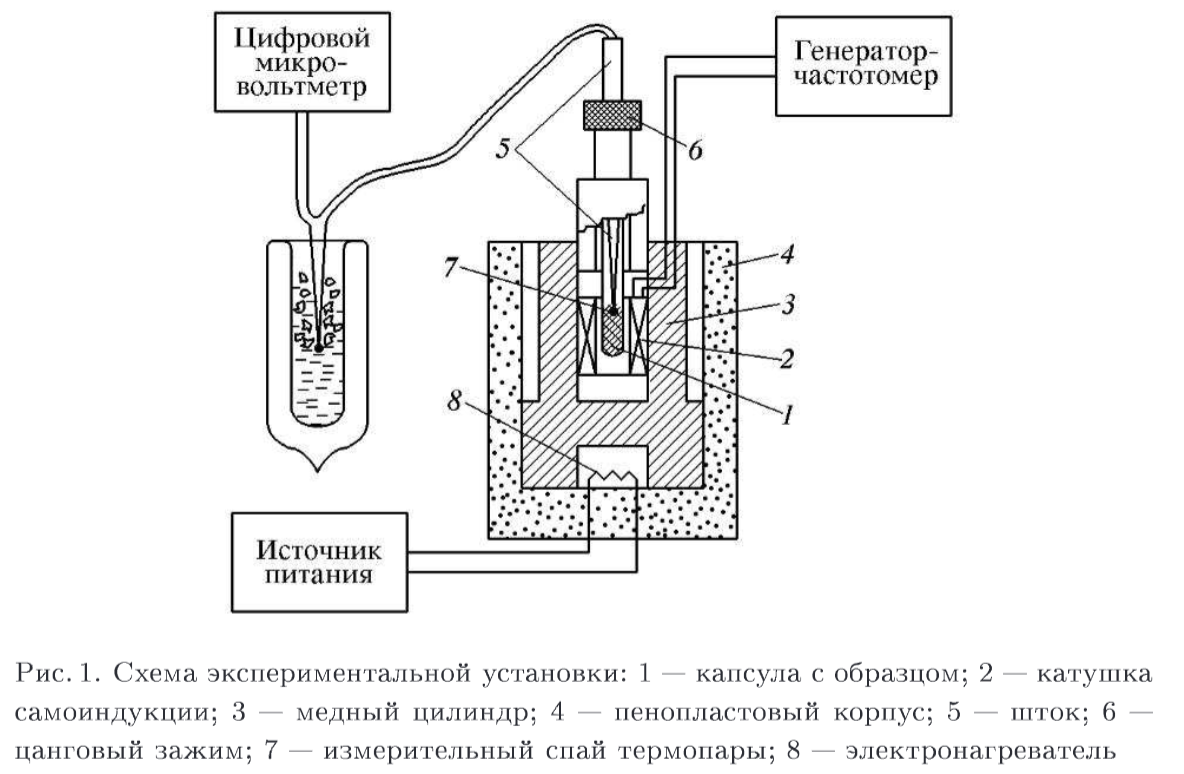
\includegraphics[scale = 0.7]{setup.png}
        \caption{}
        \label{setup}
    \end{center}
\end{figure}

Экспериментальная устанвока изображена на рис. \ref{setup}. \par 
Магнитная восприимчивость образца определяется по измерению самоиндукции, происхожящему при его введении в катушку. $L, L_0$ - самоиндукции катушки с и без образца. 

\begin{equation}
    L = \mu \frac{4 \pi n^2 S}{l} \;\;\;\;\; L_0 = \frac{4 \pi n^2}{l}
\end{equation}

\begin{equation}
    \frac{L - L_0}{L_0} = \frac{\Delta L}{L_0} = \mu -1
\end{equation}

Тк длина обраци существенно больше диаметр, то пернебрегаем размагничивающим фактором:

\begin{equation}
    \frac{L-L_0}{L_0} = \mu -1 = 4 \pi \kappa
\end{equation}

Частота колебательного контура определяется $1/f = s \pi \sqrt{LC}$:

\begin{equation}
    \frac{f^2 - f_0^2}{f^2} = 4 \pi \kappa
\end{equation}

И получаем:

\begin{equation}
    \frac{1}{\kappa} \propto \frac{f^2}{f_0^2 - f^2}
\end{equation}

Мы будем варьировать температуру от 3 до 50 $^{\circ} C$ и измерять ее будем с помощью медно-константановой термопары. 

\newpage

\section{Ход работы}

\begin{enumerate}
    \item Включим установку (Печь, генератор, нагреватель) и убедимся в исправности ее работы.
    \item Сначала будем охлаждать образец, затем будем его нагревать в заданном интервале температур 3 до 50 $^{\circ} C$. \par 
    Каждые 2-5 $^{\circ}C$ будем измерять величины $f, \; f_0$. Измерение частот производится при ватавленном и извлеченном образце соответсвенно.
    \item Построим зависимость $f^2/(f_0^2 - f^2)$ от температуры образца $T$ рис. \ref{gr1}, а все денные занесем в таблицу рис. \ref{t1}:
    
    \begin{figure}[H]
        \begin{center}
            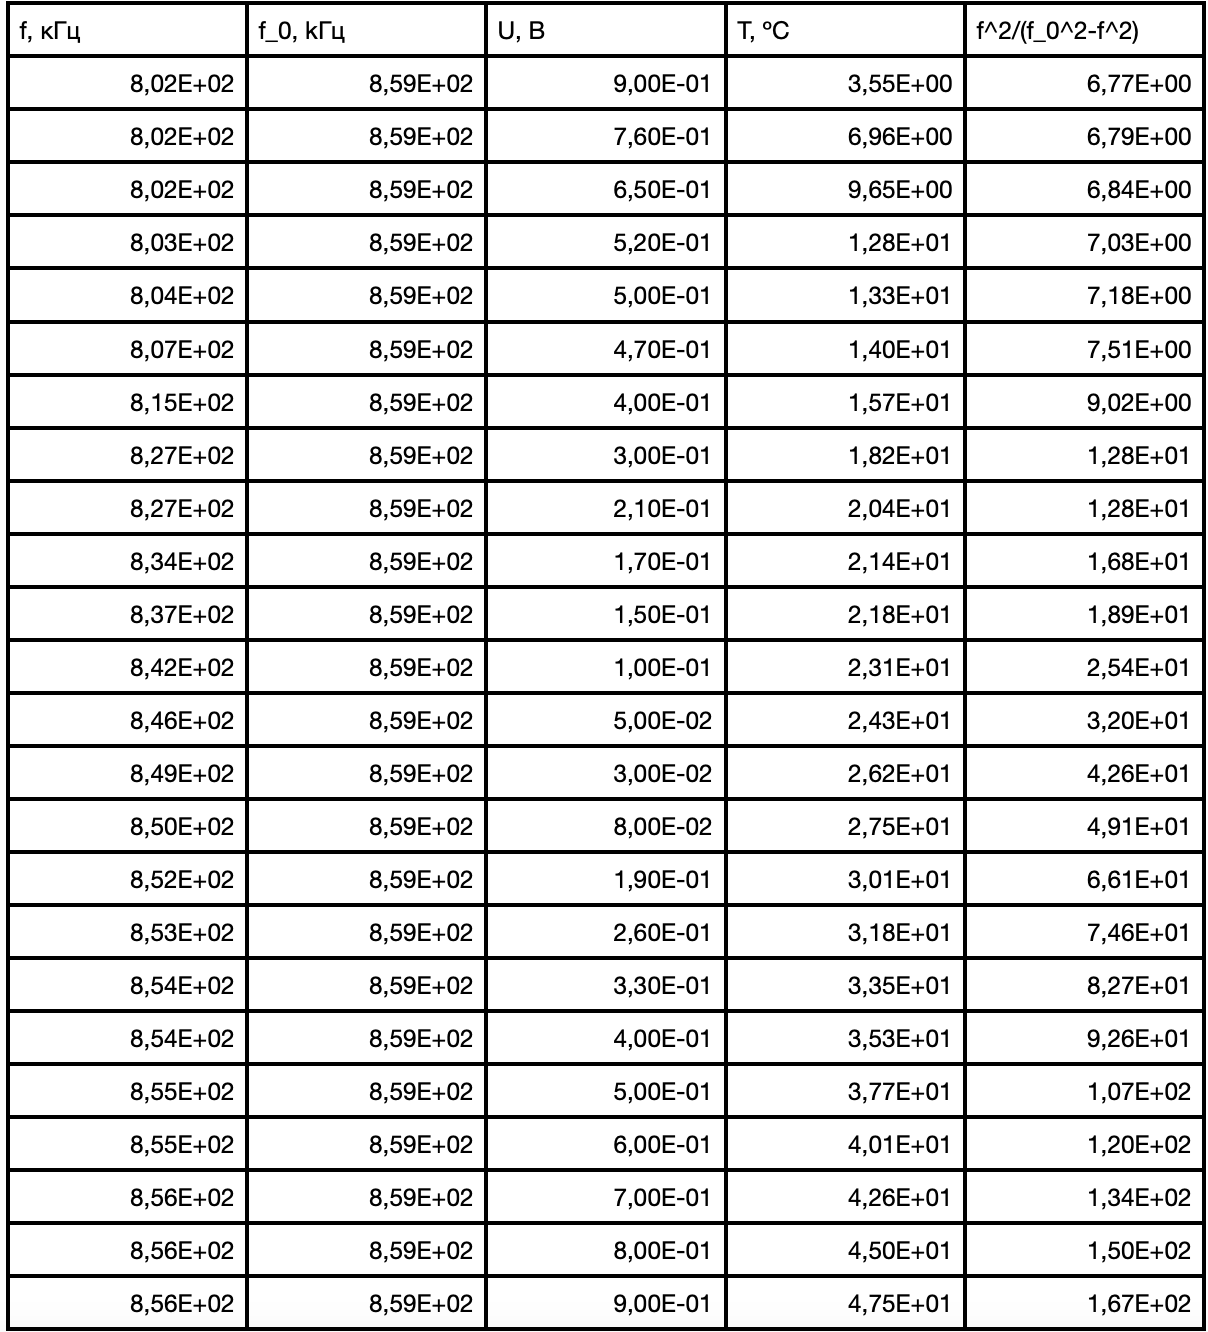
\includegraphics[scale = 0.7]{data.png}
            \caption{Данные}
            \label{t1}
        \end{center}
    \end{figure}

    \begin{figure}[H]
        \begin{center}
            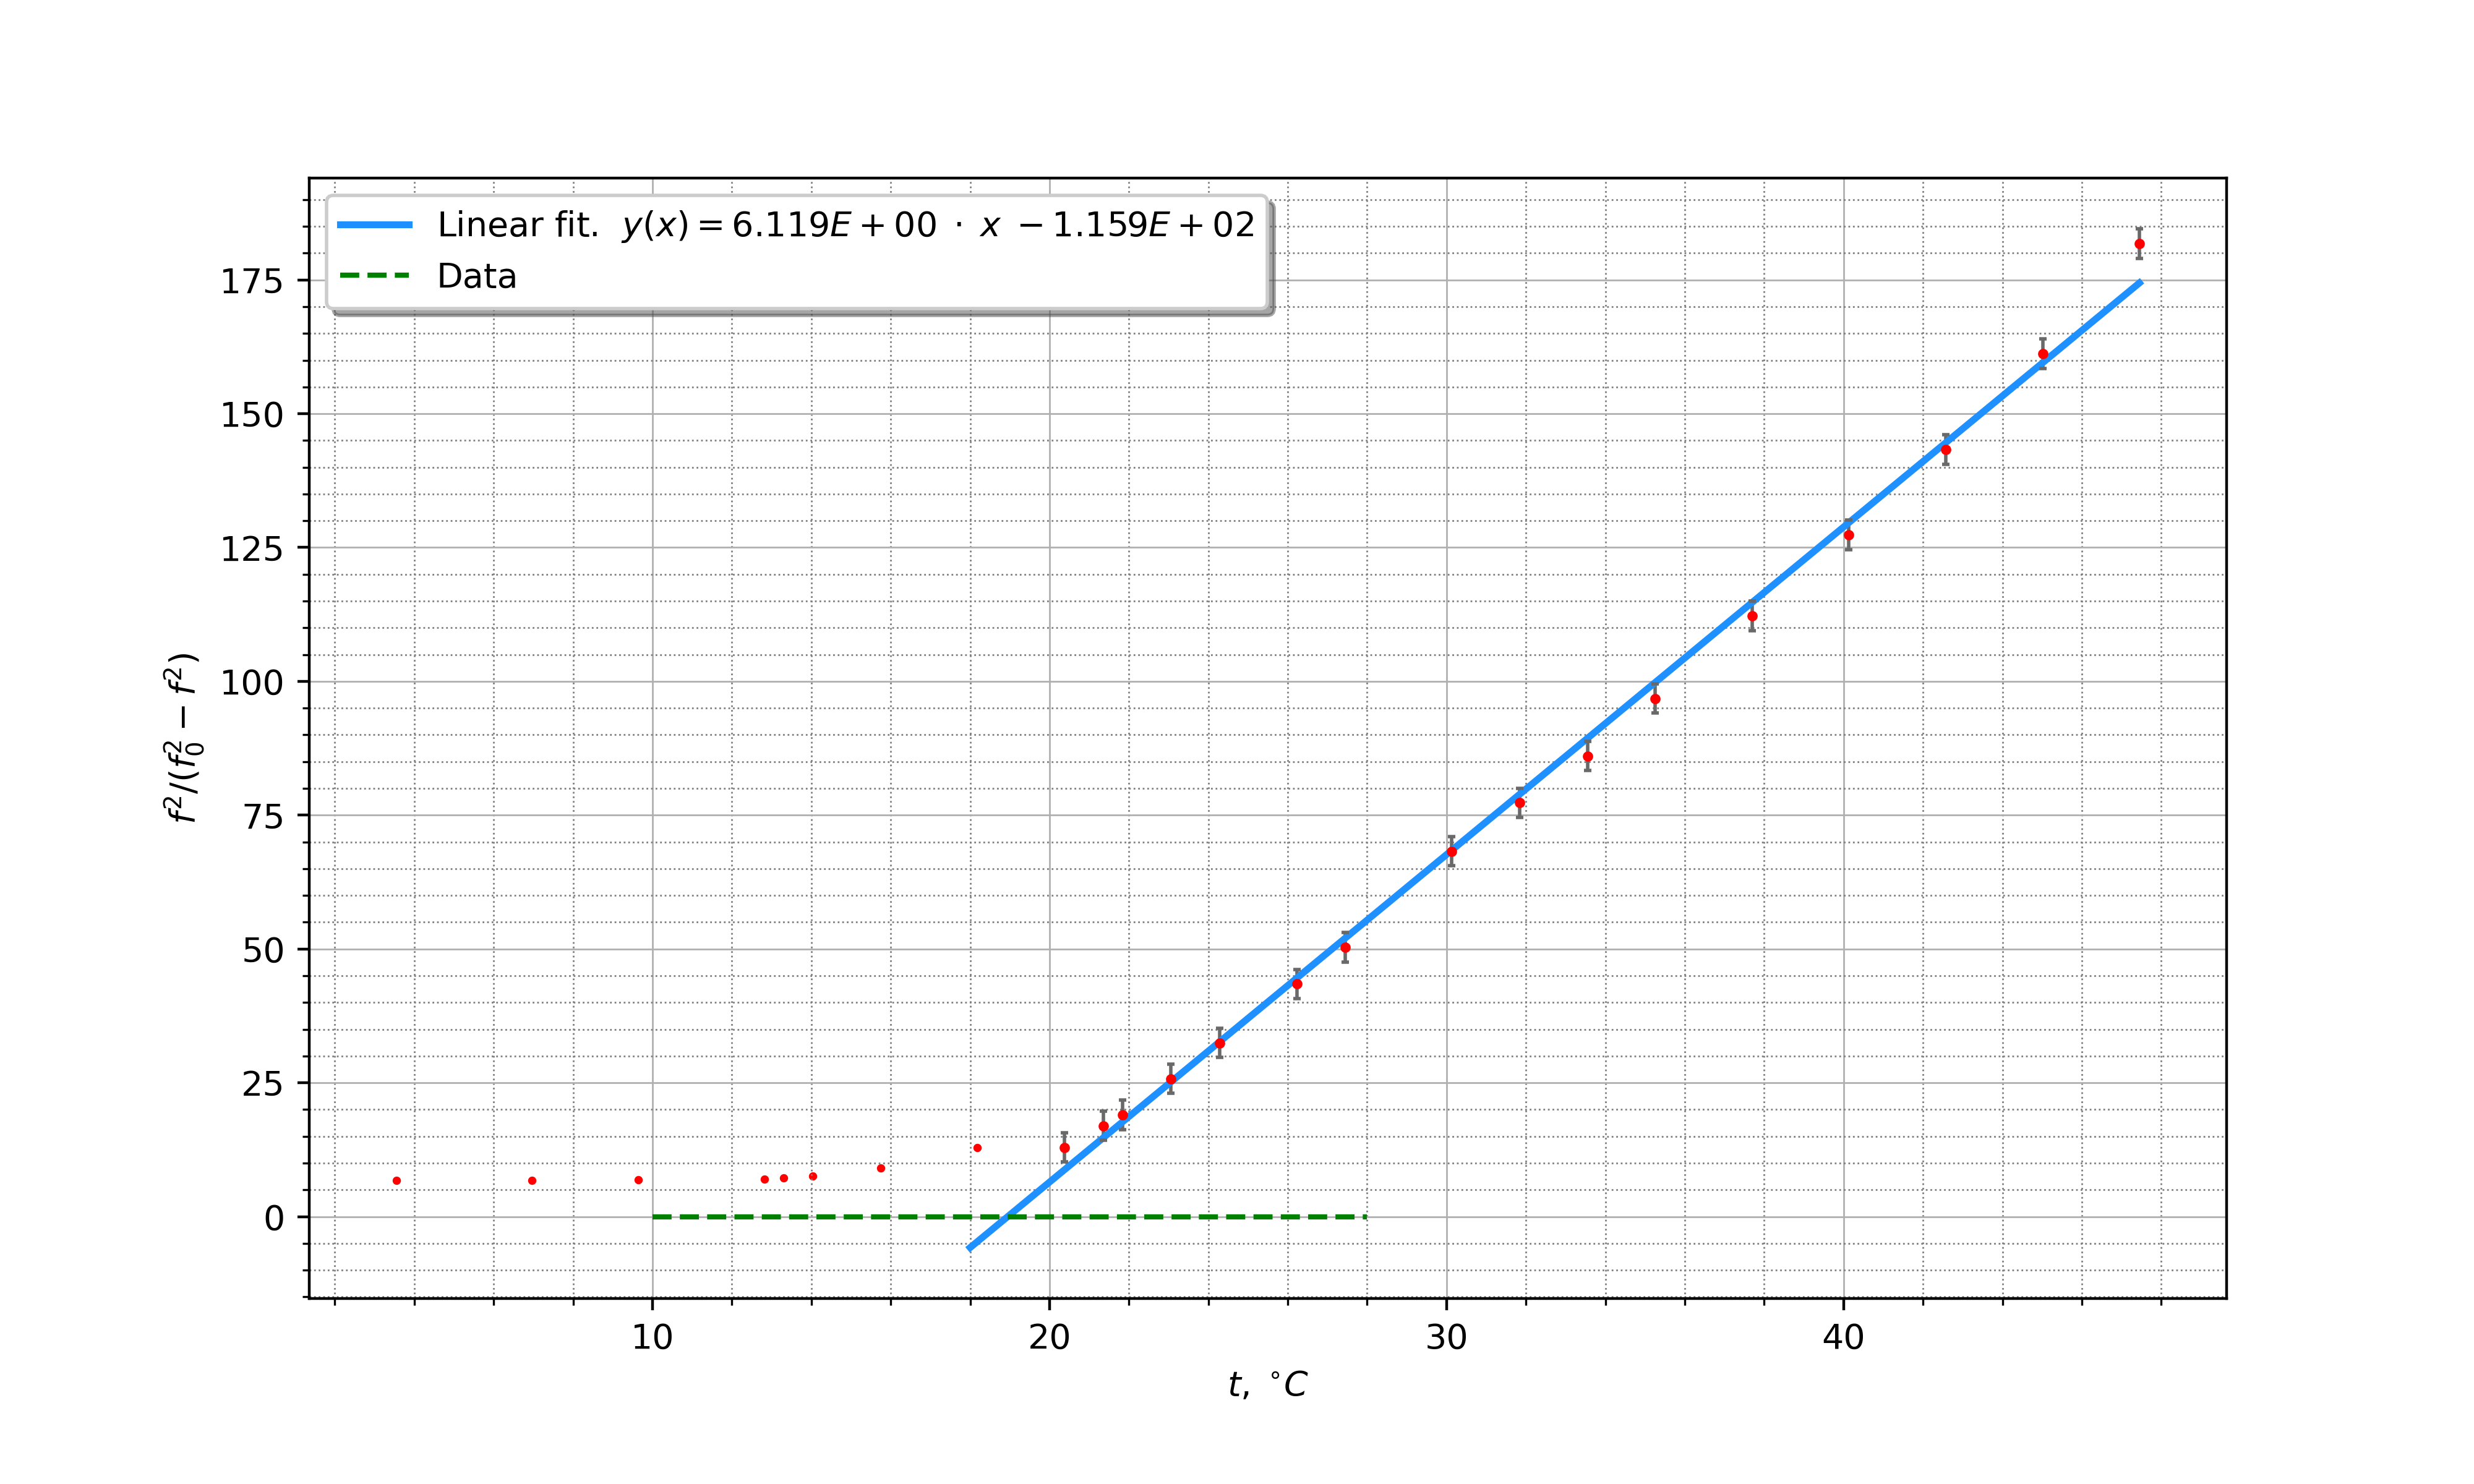
\includegraphics[scale = 0.7]{graph.png}
            \caption{Зависимость $f^2/(f_0^2 - f^2)$ от температуры образца $T$}
            \label{gr1}
        \end{center}
    \end{figure}

    По наклону графика определим точкуКюри $T_c = \Theta$. \par 

    Коэффициенты аппроксимации: $a = 6.12 \pm 0.08 \;\;\;\;\; b = 116.93 \pm 2.82$
    
    \begin{center}
        \fbox{$T_c = | \frac{b}{a} | \approx \frac{115.93}{6.12} \approx 18.95 \pm 0.03\; (^{\circ} C) \; [\pm 2.8 \%]$}
    \end{center}
       
    \item Используя формулу (16) и n = 12, $S = 7/2$ определим  $J$:

    \begin{center}
        \fbox{$J = \frac{3 k_b \Theta}{2 n S (S+1)} = (199.6 \pm 5.6) \cdot 10^{-6}\; (эВ) = 2.32 \pm 0.06 \; (K)$}
    \end{center}
    
\end{enumerate}




\section{Вывод}
\begin{itemize}
    \item В данной работе мы исследовали температурную зависимость магнитной восприимчивости ферромагнетика в парамагнитной области, зависимость отражена на графике (рис. \ref{gr1}).
    \item Определили температуру Кюри для металлического гадолиния $T_c = 291.94 \pm 0.03\; (K)$, табличное значение $T = 293.4\; (K)$. 
    \item Оценили энергию обменного взаимодействия $J = (199.6 \pm 5.6) \cdot 10^{-6}\; (эВ) = 2.32 \pm 0.06 \; (K)$
\end{itemize}



\end{document}